\documentclass[a4paper,11pt]{article}
\usepackage{multicol}
\setlength{\columnseprule}{1pt} % separation line between columns

\usepackage[top=2cm, bottom=2cm, left=2cm, right=2cm]{geometry}
\usepackage[T1]{fontenc}
\usepackage[utf8]{inputenc}
\usepackage[francais]{babel}
\usepackage{textcomp}

\usepackage{hyperref}
\hypersetup{
	colorlinks=true,       	% false: boxed links; true: colored links
	linkcolor=black,          	% color of internal links
	urlcolor=blue,           	% color of external links
	citecolor=blue
}

\usepackage{dashrule}
\usepackage{wrapfig}
\usepackage{graphicx}
\usepackage{enumitem}
\usepackage{wrapfig}
\usepackage{cancel} % diagonal strikeout
\usepackage[margin=1cm]{caption}
\usepackage{subcaption}
\setdescription{leftmargin=1cm,labelindent=0.5cm}

\usepackage{amsmath}
\usepackage{amssymb}
\usepackage{amsfonts}

\newcommand\mathd[0]{\mathrm{d}} 

\usepackage{blindtext}

% Colors
\usepackage[usenames,dvipsnames]{xcolor}
\definecolor{session_bg}{RGB}{25,25,25}
\definecolor{grey}{rgb}{0.96,0.96,0.96}
\definecolor{grey2}{rgb}{0.3,0.3,0.3}
\definecolor{dkgreen}{rgb}{0,0.6,0}
\definecolor{gray}{rgb}{0.5,0.5,0.5}
\definecolor{mauve}{rgb}{0.58,0,0.82}
\definecolor{blue}{rgb}{0,0,0.7}

% Colored frame
\usepackage{framed}
\definecolor{shadecolor}{rgb}{0.96,0.96,0.96}
\definecolor{TFFrameColor}{rgb}{0.96,0.96,0.96}
\definecolor{TFTitleColor}{rgb}{0.00,0.00,0.00}

% Redefine leftbar environment
\newlength{\leftbarwidth}
\setlength{\leftbarwidth}{1pt}
\newlength{\leftbarsep}
\setlength{\leftbarsep}{10pt}

\newcommand*{\leftbarcolorcmd}{\color{leftbarcolor}} % as a command to be more flexible
\colorlet{leftbarcolor}{gray}

\renewenvironment{leftbar}{%
    \def\FrameCommand{{\leftbarcolorcmd{\vrule width \leftbarwidth\relax\hspace {\leftbarsep}}}}%
    \MakeFramed {\advance \hsize -\width \FrameRestore }%
}{%
    \endMakeFramed
}

\usepackage{listings}
\lstset{
	numbers=left,                   % where to put the line-numbers
    language=C++,
	tabsize=4,
	frame=single,                   % adds a frame around the code
	breaklines=true,				% text wrapping
    basicstyle=\scriptsize\ttfamily,
    numberstyle=\scriptsize\ttfamily,
    backgroundcolor=\color{grey},
    showstringspaces=false,
    keywordstyle=\color{BrickRed},
    stringstyle=\color{OliveGreen},
    commentstyle=\color{grey2}\it,
	emphstyle=\color{mauve},
    stepnumber=0
}


% Title page
\title{\textbf{[PR-IT-4301] - Ivalice Commerce} \\ 
\textbf{\normalsize{Technologies JEE - Site de e-commerce}}}
\author{
	Damien Martel \\ \href{mailto:damien.martel@edu.esiee.fr}{damien.martel@edu.esiee.fr} \and
	Frédéric Nguyen \\ \href{mailto:frederic.nguyen@edu.esiee.fr}
	{frederic.nguyen@edu.esiee.fr}
}
\date{\today}

\begin{document}
\maketitle
\newpage
\tableofcontents
\newpage

\section{Contexte}

Le site a été conçu dans le cadre fictif d'un jeu vidéo. Cet univers est 
constitué d'êtres vivants contenant aussi des êtres civilisés qui constituent 
une société. \\

L'activité principale de ces personnages est celui d'aventurier. 
Ces derniers acceptent des quêtes à remplir afin d'en obtenir les récompenses. 
Ils peuvent soit travailler en solitaire, soit en guilde. \\

Une guilde est constituée de plusieurs aventuriers qui travaillent ensemble et 
partagent leurs possessions. \\

Avec ceci à l'esprit, le site de e-commerce a été développé dans le but de 
proposer tous les équipements et objets nécessaires à ces personnages pour faire 
les quêtes. Pour les guildes, une réduction sur chaque panier est appliquée 
étant donné que leurs achats se feront très souvent en grande quantité. De plus, 
cela incite les aventuriers à rejoindre des guildes pour bénéficier des 
réductions et ainsi, le site participe aussi au développement de la société.

\newpage

\section{Interface utilisateur}

Le design de ce site s'est basé sur le framework de Bootstrap qui offre un 
déploiement rapide d'un site structuré. Dans un premier temps, l'utlisateur 
fera face au portail. \\

\begin{figure}[h!]
	\centering
	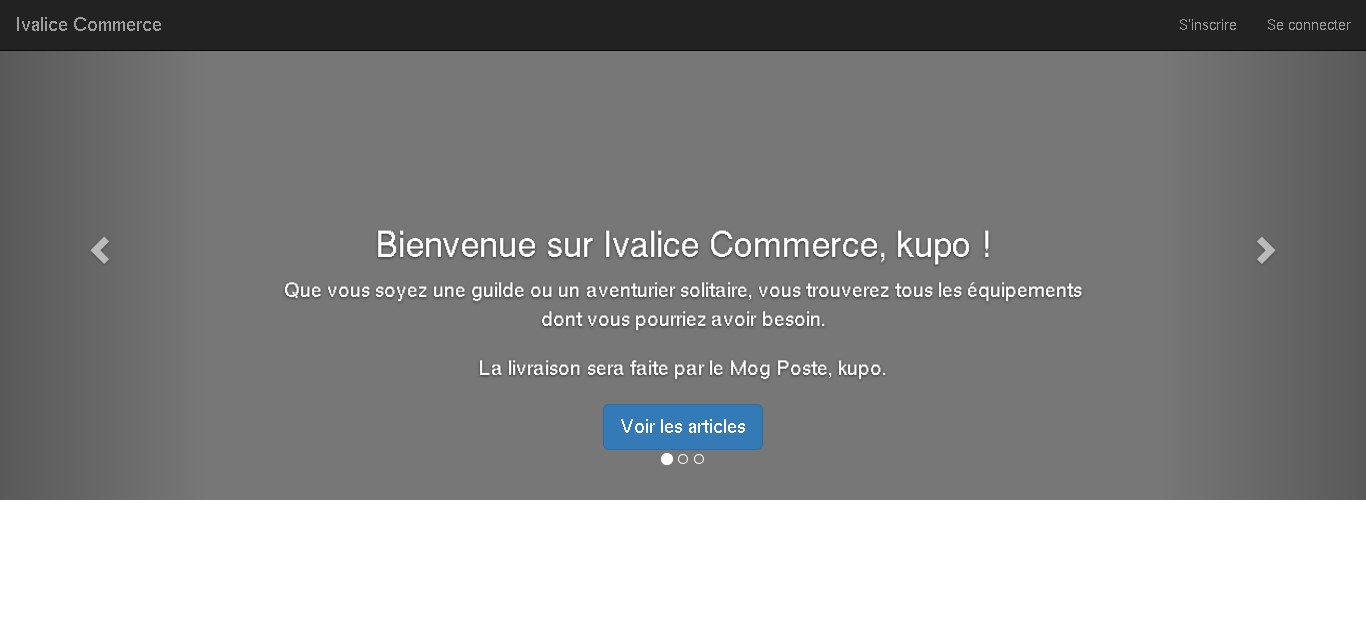
\includegraphics[width=0.8\textwidth]{img/portal.png}
	\caption{Portail}
\end{figure}

Cette page lui présente rapidement les services du site 
sur une vitrine et donne des accès rapides à d'autres pages (une liste de produits pour les 
non membres, un lien vers la page d'inscription ou de connexion). \\

\begin{figure}[h!]
	\centering
	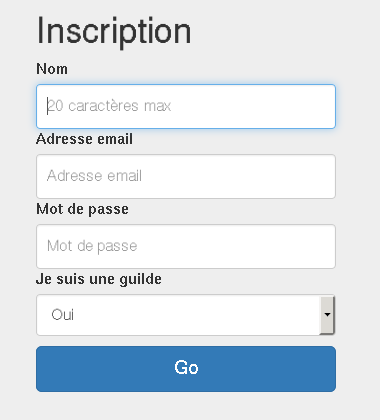
\includegraphics[width=0.3\textwidth]{img/signup.png}
	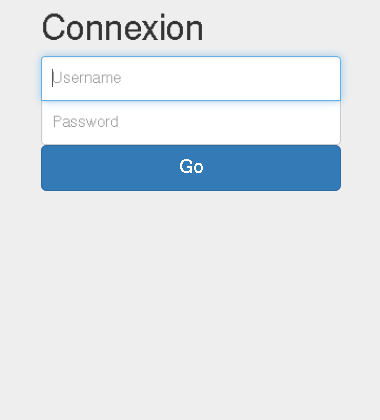
\includegraphics[width=0.3\textwidth]{img/login.png}
	\caption{Formulaire d'inscription et de connexion}
\end{figure}

Une fois connecté, on arrive à une page d'index qui affiche la liste des produits. 
Il y a un menu latéral qui lui permet de filtrer la liste des produits. Dans le 
tableau récapitulant les produits, il se trouve des boutons d'action qui 
permettent d'ajouter ou de retirer une unité de ce produit dans le panier. \\

\begin{figure}[h!]
	\centering
	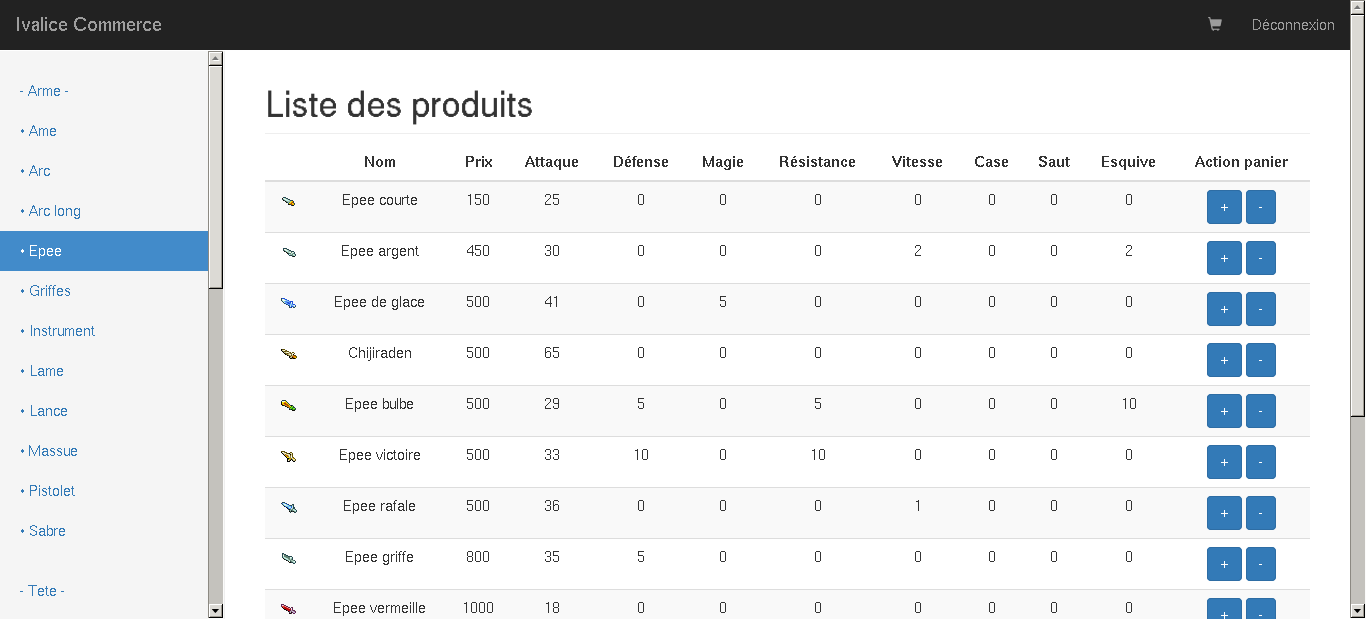
\includegraphics[width=0.8\textwidth]{img/index.png}
	\caption{Liste des produits filtrée (Epée)}
\end{figure}

\newpage
Sur la page du panier, les produits sélectionnés par l'utilisateur sont listés 
et le prix total est indiqué. Si le membre est une guilde, le total serait 
indiqué en rouge avec une réudction de 5\%. Il lui est aussi possible de 
retirer des produits directement à partir du panier. \\

\begin{figure}[h!]
	\centering
	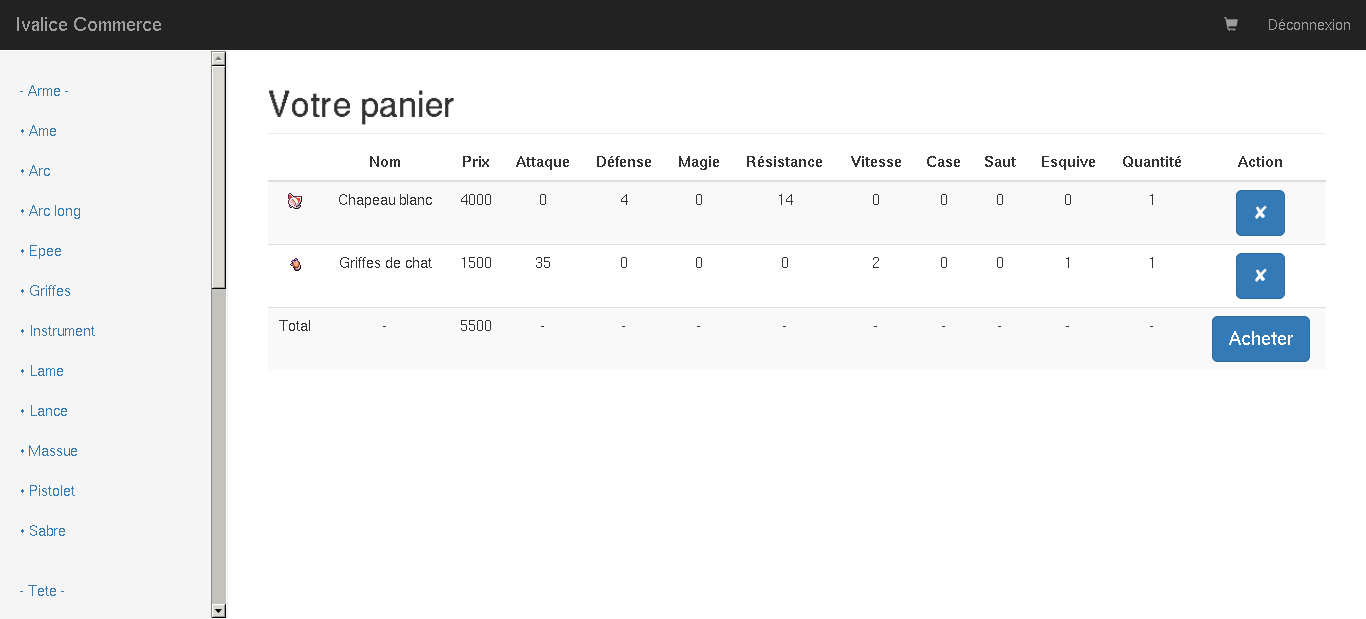
\includegraphics[width=0.8\textwidth]{img/cart.png}
	\caption{Panier d'un membre non guilde}
\end{figure}

Il ne reste donc plus qu'à acheter l'ensemble des produits dans le panier. On 
arrive sur une page confirmant que l'achat a été effectué. Le panier de 
l'utilisateur est donc vidé à l'occasion. \\

\begin{figure}[h!]
	\centering
	
\includegraphics[width=0.6\textwidth]{img/buy.png}
	\caption{Confirmation d'achat}
\end{figure}

Enfin, si un utilisateur essaie de s'inscrire avec des identifiants déjà 
existants, ou s'il se connecte avec des mauvais identifiants, il sera renvoyé au 
portail avec des messages d'erreur. \\

\begin{figure}[h!]
	\centering
	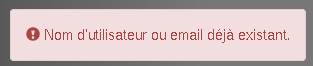
\includegraphics{img/trysignup.png}
	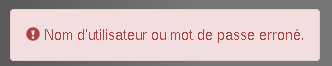
\includegraphics{img/trylogin.png}
	\caption{Messages d'erreur pour inscription ou connexion échouée}
\end{figure}


\newpage

\section{Structure du projet}

\subsection{Répertoires}

Le projet se divise en deux grands répertoires principaux : le répertoire pour 
les sources java et le répertoire pour les sources web.

\begin{description}
	\item[Web pages] \hfill \\
		css \\
		fonts \\
		img \\
		js \\
		jsp
	\item[Src] \hfill \\
		controller \\
		bean \\
		src
\end{description}

\subsection{web.xml}

\lstinputlisting{../web/WEB-INF/web.xml}

\subsection{Navigation des pages web}

L'ensemble des pages de navigation du site comporte un portail, une page 
d'inscription, une page de connexion, une page listant tous les produits servant 
de vitrine pour les utilisateurs non connectés et un panier. \\

L'index est la page principale une fois l'utilisateur connecté. Elle permet de 
navigeur dans les produits du sites et de faire des recherches filtrées par 
type ou catégorie. \\

D'autres fichiers jsp existants sont utilisés dans les pages de navigation en 
tant que partie de page html à inclure car elles permettent de compléter des 
contenus en fonction de la session utilisateur ou alors d'avoir des structures 
présentent dans toutes les pages à include. Ceci permet une meilleur modularité 
au niveau du développement.

\subsection{Architecture MVC2}

Pour programmer un site bien structuré et modulaire, nous avons suivi le 
design pattern MVC adapté pour un projet JEE. Ce dernier consiste à séparer trois 
entités : le Model, la View et le Controller. \\

Le concept de base veut que le Controller se charge des modifications dans le 
Model et d'actualiser la View. Le rôle du Model n'est que de stocker et de 
fournir les procédés de modification de données au Controller. La View est ce 
que voit les utilisateurs. Elle affiche l'interface graphique en fonction de ce 
qu'a demandé le Controller et en fonction des données du Model. \\

Dans le cadre des technologies J2EE, il est souhaité que le Controller soit 
implémenté par une Servlet unique qui sert d'aiguilleur vers les différentes 
pages du site qui sont des View écrites en JSP. Il existe d'autres servlets 
dans notre projet mais qui ne servent seulement à exécuter les requêtes 
déléguées par le Controller.\\

Le Model est représenté par des classes JavaBeans. Une classe JavaBean est une 
classe Java suivant des directives strictes. Il ne doit pas avoir de 
constructeur et ne doit contenir que les attributs, les getter et les setter. 
Les Javabeans permettent de faciliter l'utilisation de la base de données. \\

De manière générale, un navigateur commence par envoyer une requête au 
Controller qui va rediriger l'utilisateur vers la View correspondante et si 
besoin, utiliser le Model pour compléter le contenu de la View qui est renvoyée 
en guise de réponse au navigateur.

\newpage

\section{Modèle 3-tiers}
En plus du modèle MVC de base, nous avons choisis de suivre un modèle \emph{3 tiers} plus adapté aux sites internet.
Ce modèle permet d'obtenir un site bien structuré et modulaire.

Ce design est composé de 3 couches,
La couche présentation, métier et donnée.

\subsection{La couche Présentation}
Cette couche est le front-end de notre application, elle correspond au code html générer et vue par l'utilisateur, elle touche tout ce qui est navigation dans le site, ergonomie et effet visuel.
Cette couche est donc générer par nos JSP, et fourni a l'utilisateur l'interface visible par son navigateur.
Elle est aussi responsable de fournir des méthodes d'accès au contrôleur afin de pouvoir naviguer sur notre site.
Elle crée des formulaires ou des liens permettant à l'utilisateur d'envoyer des requêtes à notre contrôleur.

\subsection{La couche Métier}
Le couche métier regroupe toute la logique de notre application, c'est ici que nous retrouverons notre MVC2.

Ce dernier consiste à séparer trois 
entités : le Model, la View et le Controller. \\

Le concept de base veut que le Controller se charge des modifications dans le 
Model et d'actualiser la View.
Le rôle du Model n'est que de stocker et de
fournir les procédés de modification de données au Controller. La View est ce que voit les utilisateurs.
Elle affiche l'interface graphique en fonction de ce 
qu'a demandé le Controller et en fonction des données du Model. \\


\subsubsection{Controller}
Dans le cadre des technologies J2EE, il est souhaité que le Controller soit implémenté par une Servlet unique qui sert d'aiguilleur vers les différentes 
pages du site qui sont des View écrites en JSP. Il existe d'autres servlets 
dans notre projet mais qui ne servent seulement à exécuter les requêtes déléguées par le Controller.\\

\subsubsection{Model}
Le Model est représenté par des classes JavaBeans. Une classe JavaBean est une 
classe Java suivant des directives strictes. Il ne doit pas avoir de 
constructeur et ne doit contenir que les attributs et des mutators (les getter et les setter).
Les Javabeans permettent de faciliter l'utilisation de la base de données. \\
Ce module permet la liaison avec la base de donnée en utilisant l'api de la couche donnée, le module est capable de récupérer des information ou en stocker au travers des Java beans

\subsubsection{View}
De manière générale, un navigateur commence par envoyer une requête au 
Controller qui va rediriger l'utilisateur vers la View correspondante et si 
besoin, utiliser le Model pour compléter le contenu de la View qui est renvoyée en guise de réponse au navigateur.\\
C'est ce module qui permet la liaison avec la couche présentation à l'aide des jsp.
Elle génère dynamiquement la page envoyer à l'utilisateur en fonction d'information obtenu par le contrôleur.

\subsection{La couche Donnée}
La couche donnée correspond a tout les données statique, c'est a dire stocker dans une base de donnée la plupart du temps.
Elle est composé de notre base de donnée Derby ainsi que de la classe DBManager fournissant des méthodes d'accès.

Sont rôle est de fournir les données à la couche métier au travers des javabeans.
Elle permet de les peupler lorsque la couche métier demande des donnée et de les stocker lorsque cela est necessaire.

\newpage

\section{Structure de base de données}

La base de données contient deux tables : Member et Item. \\

Member contient les données des utilisateurs fournis au moment de l'inscription. 
La table se présente comme suivant :

\begin{description}
	\item[Name] VARCHAR(20) UNIQUE NOT NULL
	\item[Password] CHAR(128) NOT NULL
	\item[Email] VARCHAR(255) NOT NULL PRIMARY KEY
	\item[Guild] BOOLEAN NOT NULL
\end{description}

Le mot de passe passe par un algorithme de hachage avant d'être stocké dans 
la base de données. \\

La table Item comporte toutes les informations concernants les produits à 
vendre ainsi que le chemin de fichier vers l'image correspondant à chaque 
produit.

\begin{description}
	\item[Name] VARCHAR(30) NOT NULL PRIMARY KEY
	\item[Type] VARCHAR(30) NOT NULL
	\item[Category] VARCHAR(30) NOT NULL
	\item[Price] NUMERIC(7,0) NOT NULL
	\item[Attack] NUMERIC(3,0) NOT NULL
	\item[Defense] NUMERIC(3,0) NOT NULL
	\item[Magic] NUMERIC(3,0) NOT NULL
	\item[Resistance] NUMERIC(3,0) NOT NULL
	\item[Speed] NUMERIC(3,0) NOT NULL
	\item[Move] NUMERIC(3,0) NOT NULL
	\item[Evasion] NUMERIC(3,0) NOT NULL
	\item[Path] VARCHAR(255) NOT NULL
\end{description}

Le script pour créer les tables et les remplir se trouvent à 
\href{https://github.com/fmutix/I-Commerce/tree/master/script}
{https://github.com/fmutix/I-Commerce}

\newpage

\section{Data Access Object}

La Data Access Object fournit une interface avec la base de données. Dans le 
projet, elle prend la forme d'une classe java intégrant JDBC qui contient les 
méthodes de communication avec une base de données. \\

Ici, elle peut :

\begin{itemize}
	\item se connecter ou se déconnecter à la base de données
	\item ajouter un membre
	\item récupérer les données d'un membre
	\item récupérer les données d'un item
	\item récupérer tous les items de la base de données (trié ou non)
	\item récupérer le type ou la catégorie d'un item
\end{itemize}

\newpage

\section{Code source}

Les sources du projet se trouve sur notre dossier Git sur 
\href{https://github.com/fmutix/I-Commerce}
{https://github.com/fmutix/I-Commerce}.

\newpage

\section{Techniques JEE employées}

Pour développer le site de e-commerce, nous avons donc utilisé du Java, les 
langages web (HTML/CSS/Javascript), le JSP, les EL et le JSTL. \\

Le Java nous a permis de faire entièrement la partie back-end, ce langage 
constitue donc une majeure partie du projet. \\

Le JSP permet d'intégrer facilement du code java dans les sources web et 
permet d'éviter de faire les écritures sur l'affichage web dans les servlets 
(PrinterWriter), ce qui est déprécié. De plus, nous utilisons les EL afin 
d'avoir une syntaxe plus simple et de pouvoir utiliser les Javabean plus 
facilement. Pour compléter ces deux langages, nous avont aussi intégré du JSTL. 
Il s'agit d'une importation de bibliothèque qui permet d'utiliser plus de 
fonctionnalités dans le JSP. \\

Pour gérer la connexion des utilisateurs et de garder des données durant la 
navigatation, nous avons utilisé les techniques d'utilisation de sessions. 
Cette gestion fait intervenir toutes les techniques précédentes. Il faut 
seulement préciser un détail de scope de session et travailler sur cette 
session dans le code.

\newpage

\section{Conclusion}

Cet atelier de technologies JEE a été une opportunité pour nous de découvrir 
des outils pour créer un site de e-commerce dans le cadre de notre projet. Cela 
pour permettra aussi de pouvoir créer d'autres types de sites dont l'utilisation 
des technologies JEE sont efficaces. \\

Durant ce projet, nous n'avons pas eu de réelles difficultés, mis à part 
lorsque nous devons définir certains concepts comme la DAO et sa place dans 
les architectures trois tiers. \\

L'organisation de l'équipe s'est faite avec à l'aide de Trello, une application 
web qui permet de classer nos tâches par catégories. Nous avons utilisé cet 
outils dans une perspective de méthode agile afin d'avoir toujours un résultat 
présentatble. En ce qui concerne l'organisation de la programmation, nous 
avons utilisé le gestionnaire de version Git. Ce qui noous a grandement aidé 
pour développer sur le projet simultanément.


\end{document}
